\documentclass[utf8]{ctexart}

\usepackage[a4paper,left=1.25in,right=1.25in,top=1in,bottom=1in]{geometry}
\usepackage{listings}
\usepackage{graphicx}
\usepackage{caption}
\usepackage{subfigure}
\usepackage{booktabs}
\usepackage{amsmath}
\usepackage{amsthm}
\usepackage{amsfonts}
\usepackage{float}
\usepackage{indentfirst}
\usepackage{tikz}
\usetikzlibrary{shapes,arrows}
\usetikzlibrary{shapes.geometric, arrows}
\usepackage{algorithm}
\usepackage{algorithmic}
\usepackage{newclude}
\usepackage[perpage]{footmisc}

\graphicspath{ {images/} }
\raggedbottom	% 令页面在垂直方向向顶部对齐
\renewcommand\qedsymbol{QED}
\newcommand{\sign}[1]{\mathrm{sgn}(#1)}
\everymath{\displaystyle}   % 行内公式采用行间公式格式排列
\pagestyle{plain}

\title{《计算机辅助几何设计》第三次作业}
\author{姓名:殷文良\qquad 学号:12435063}
\date{\today}

\begin{document}
\maketitle
\ctexset { section = { format={\Large \bfseries } } }

\section*{思考题 1}
\subsection*{1.}
\begin{proof}
    定义函数$q(t)=(x-t)^n$,其中$x$是自由参数。由于$q(t)\in \mathbb{P}_n$,根据插值多项式的唯一性以及Cauchy余项定理,
    我们有$p_n(q;t) \equiv q(t)$。
    在$t_0,\dots,t_n$处对$q(x)$进行Lagrange插值,则有
    $$
    (x-t)^n \equiv \sum_{k=0}^nL_k^n(t|t_0,\dots,t_n)(x-t_k)^n.
    $$
\end{proof}
\subsection*{2.}
采用不同的参数化方法实现Lagrange曲线插值,分别为均匀参数化、累积弦长参数化和切比雪夫累积弦长参数化\footnote{参考《数据插值中的参数化新方法》},并比较插值效果。
\begin{itemize}
    \item 2维:$p_0 = (-1,0)',
    p_1 = (0,1)',
    p_2 = (3,3)',
    p_3 = (1,0)',
    p_4 = (0,-1)'.$

    \begin{figure}[H]
        \centering
        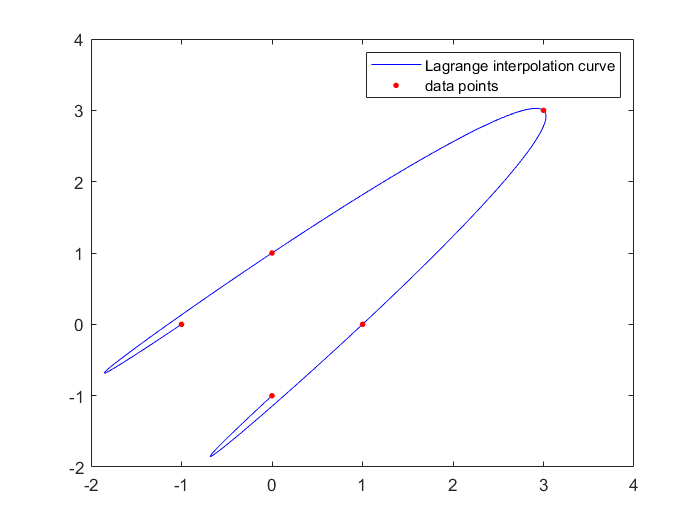
\includegraphics[width=0.8\textwidth]{lagrange_2d_uniform.png}
        \label{fig1}
        \caption{均匀参数化}
    \end{figure}
    \begin{figure}[H]
        \centering
        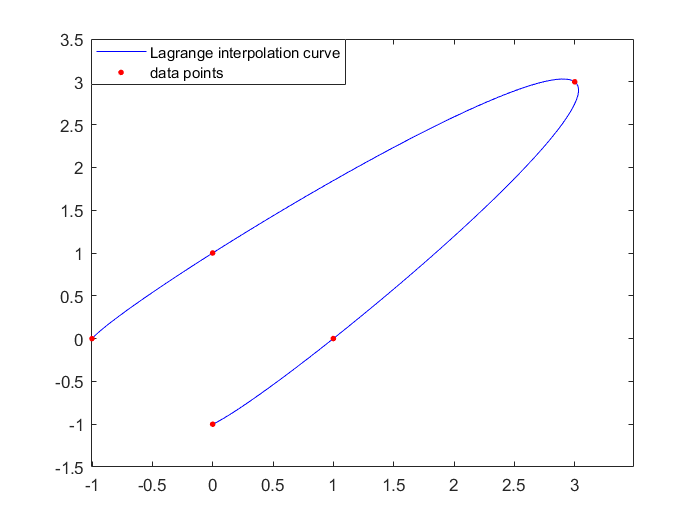
\includegraphics[width=0.8\textwidth]{lagrange_2d_chord.png}
        \label{fig2}
        \caption{累积弦长参数化}
    \end{figure}
    \begin{figure}[H]
        \centering
        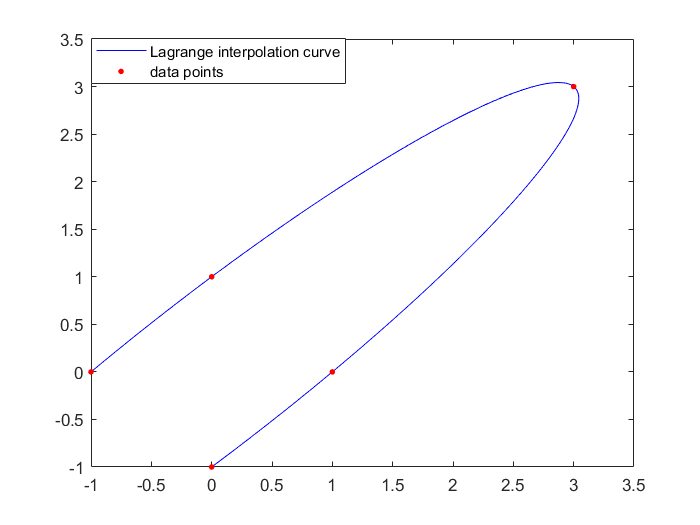
\includegraphics[width=0.8\textwidth]{lagrange_2d_cheby.png}
        \label{fig3}
        \caption{切比雪夫累积弦长参数化}
    \end{figure}

    \item 3维:$p_0 = (-1,0,0)',
    p_1 = (0,2,1)',
    p_2 = (3,3,3)',
    p_3 = (1,0,2)',
    p_4 = (0,-1,0)'.$
    \begin{figure}[H]
        \centering
        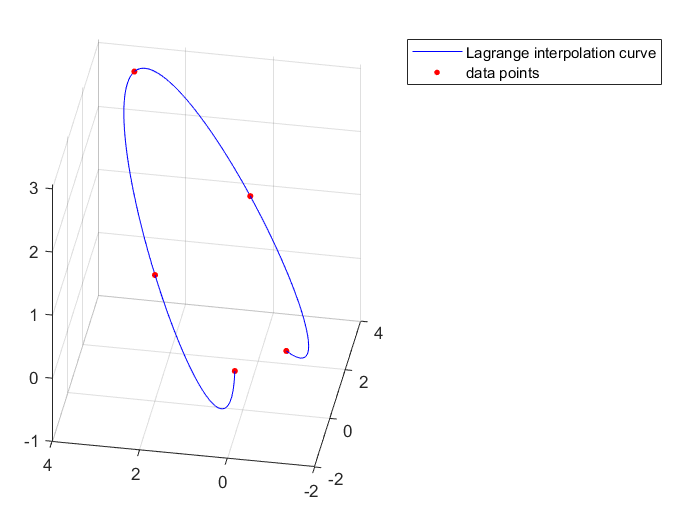
\includegraphics[width=0.8\textwidth]{lagrange_3d_uniform.png}
        \label{fig4}
        \caption{均匀参数化}
    \end{figure}
    \begin{figure}[H]
        \centering
        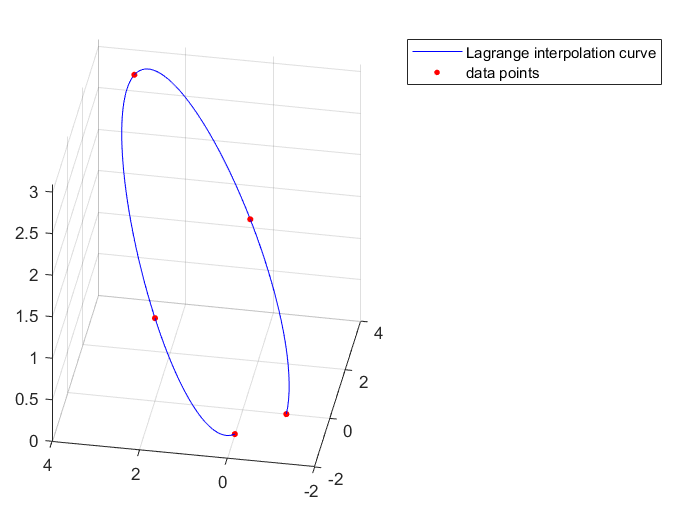
\includegraphics[width=0.8\textwidth]{lagrange_3d_chord.png}
        \label{fig5}
        \caption{累积弦长参数化}
    \end{figure}
    \begin{figure}[H]
        \centering
        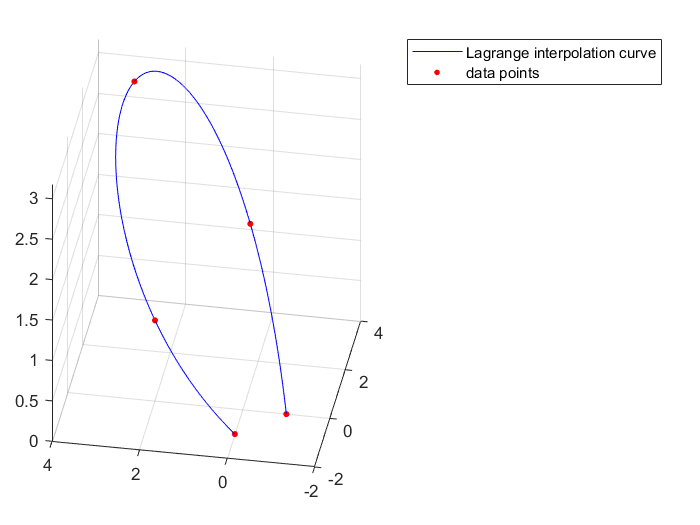
\includegraphics[width=0.8\textwidth]{lagrange_3d_cheby.png}
        \label{fig6}
        \caption{切比雪夫累积弦长参数化}
    \end{figure}
\end{itemize}
\begin{figure}[H]
    \centering
    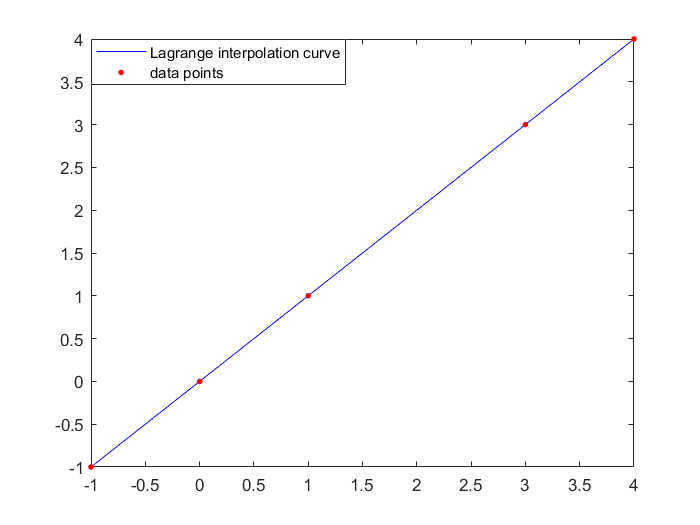
\includegraphics[width=0.8\textwidth]{lagrange_linear.png}
    \label{fig7}
    \caption{型值点共线时得到的插值曲线是直线}
\end{figure}

\section*{思考题 2}
\subsection*{1.}
\begin{proof}
    $n=0$时显然成立,现在考虑$n>0$的情形。\\
    令$f(t)=\frac{1}{x-t},g(t)=x-t$,其中$x$是参数。于是,$(fg)[t_0,\dots,t_n] = (1)[t_0,\dots,t_n]=0$。
    另一方面,根据Leibniz公式以及差商的性质,我们有
    \begin{equation*}
        \begin{aligned}
            (fg)[t_0,\dots,t_n] &= \sum_{k=0}^nf[t_0,\dots,t_k]\cdot g[t_k\dots,t_n]\\
            &= \sum_{k=0}^n\frac{1}{x-t}[t_0,\dots,t_k]\cdot (x-t)[t_k,\dots,t_n]\\
            &= \frac{1}{x-t}[t_0,\dots,t_{n-1}]\cdot (x-t)[t_{n-1},t_n] + \frac{1}{x-t}[t_0,\dots,t_{n}]\cdot (x-t)[t_n]\\
            &= -\frac{1}{x-t}[t_0,\dots,t_{n-1}] + \frac{1}{x-t}[t_0,\dots,t_{n}]\cdot(x-t_n).
        \end{aligned}
    \end{equation*}
    记$F(n) = \frac{1}{x-t}[t_0,\dots,t_{n}]$,于是$F(n) = \frac{1}{x-t_n}F(n-1)$。又因为$F(0)=\frac{1}{x-x_0}$,可得
$$
\frac{1}{x-t}[t_0,\dots,t_{n}] = F(n) = \frac{1}{(x-t_0)\cdots(x-t_n)}.
$$
\end{proof}

\subsection*{2.}
\begin{proof}
    只需证明$P(t)$是单项式时结论成立,从而根据差商的线性性质可得$P(t)$是多项式时的情形成立。\\
    设$P(t)=t^m(m> n)$($m\leq n$的情形是显然的),通过差商的定义和数学归纳法容易证明$P(t)$是关于$t_0,\dots,t_n$的完全对称多项式。
\end{proof}

\section*{思考题 3}
\subsection*{1.}
\begin{proof}
    记$f_i=f(t_i)$,先证明
    $$
    \Delta^nf_i = \sum_{k=0}^n(-1)^{n-k}\binom{n}{k}f_{i+k}.
    $$
    对于$n=1$,$\Delta f_i = f_{i+1} -f_i$,显然成立。假设结论成立,根据归纳步骤,我们有
$$
\begin{aligned}
\Delta^{n+1}f_i &= \Delta\Delta^nf_i = \Delta\left( \sum_{k=0}^n(-1)^{n-k}\binom{n}{k}f_{i+k}\right)\\
&= \sum_{k=0}^n(-1)^{n-k}\binom{n}{k}f_{i+k+1} - \sum_{k=0}^n(-1)^{n-k}\binom{n}{k}f_{i+k}\\
&= \sum_{k=1}^n(-1)^{n+1-k}\binom{n}{k-1}f_{i+k} + f_{i+n+1} \\
&\quad + \sum_{k=1}^n(-1)^{n-k+1}\binom{n}{k}f_{i+k} + (-1)^{n+1}f_i\\
&= \sum_{k=0}^{n+1}(-1)^{n+1-k}\binom{n+1}{k}f_{i+k}.
\end{aligned}
$$
于是当$i=0$时,便有$\Delta^{n}F(t_0) = \sum_{k=0}^{n}(-1)^{n+1-k}\binom{n}{k}F(t_k)$成立。
\end{proof}

\subsection*{2.}
\begin{proof}
    记$l_n(t)=\prod_{i=0}^n(t-t_i)$,则$l_m'(t_k) = \prod_{i=0,i\ne k}^n(t_k-t_i)$。
    于是,由$t_k-t_i = (k-i)\Delta t$可得, 
    $$
    l_n'(t_k) = \prod_{i=0,i\ne k}^n (k-i)\Delta t = (\Delta t)^nk!(n-k)!(-1)^{n-k}.
    $$
    因此,我们有
    $$
    F[t_0,\dots,t_n] = \sum_{k=0}^n\frac{F(t_k)}{l_n'(t_k)} = \sum_{k=0}^n\frac{(-1)^{n-k}F(t_k)}{k!(n-k)!(\Delta t)^n} 
    = \frac{1}{n!(\Delta t)^n}\sum_{k=0}^n(-1)^{n-k}\binom{n}{k}F(t_k) = \frac{\Delta^n F(t_0)}{n!(\Delta t)^n}.
    $$
\end{proof}


\end{document}
